% !TeX spellcheck = en_GB
\chapter{System Modelling} \label{chap3}
	\section{Introduction}
	\section{OFDM System} \label{sec3:OFDM System specification}
		\subsection{Wavelet-Based OFDM System}
			\begin{verbatim}
			s = conv(dyadup(xa),f0) + conv(dyadup(xd),f1);
			\end{verbatim}
			while the analysis side (receiver) is implemented as:
						\begin{verbatim}
						xa =  dyaddown(conv(s,h0))
						xd =  dyaddown(conv(s,h1))
						\end{verbatim}
			where the command \verb|`conv'| is a convolution operation, \verb|`dyadup'| and \verb|`dyaddown'|  are, respectively, upsampling and downsampling (by 2) operations, \verb|f0| and \verb|f1| are the lowpass and the highpass filter coefficients, respectively, of the synthesis side; \verb|h0| and \verb|h1| are the lowpass and highpass filter coefficients of the analysis side. All these terms are discussed in Section \ref{sec2:W-OFDM}.
			\subsubsection{Haar}
			\subsubsection{Daubechies-4 (db2)}
			\subsubsection{Biorthogonal-4.4 (bior4.4)}
			Figure~\ref{fig3:bior_info} shows properties of this wavelet.
		\begin{figure}[p]
		\centering
		\subfloat[Analysis scaling function $ \phi_1(t) $]{\label{subfig3:bior_phi1}{\includegraphics [width=0.45\textwidth]{./chap_3/bior_phi1}}} \hfill
		\subfloat[Analysis wavelet function $ w_1(t) $]{\label{subfig3:bior_w1}{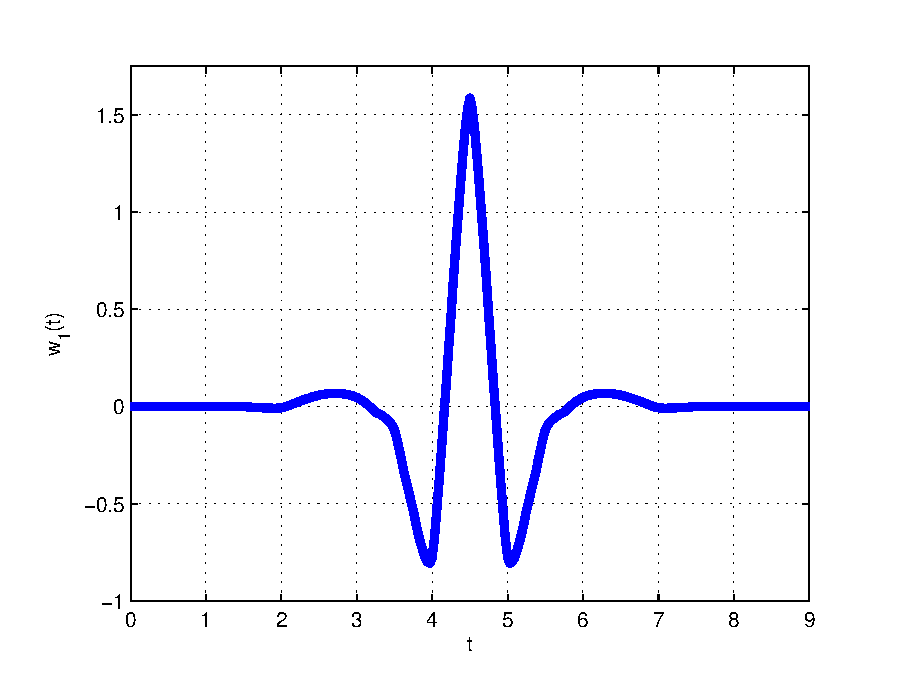
\includegraphics[width=0.45\textwidth]{./chap_3/bior_w1}}}\\
		\subfloat[Analysis low-pass filter $ h_0 $]{\label{subfig3:bior_h0}{\includegraphics[width=0.45\textwidth]{./chap_3/bior_h0}}}\hfill
		\subfloat[Analysis high-pass filter $ h_1 $]{\label{subfig3:bior_h1}{\includegraphics [width=0.45\textwidth]{./chap_3/bior_h1}}}\\
		\subfloat[Synthesis scaling function $ \phi_2(t) $]{\label{subfig3:bior_phi2}{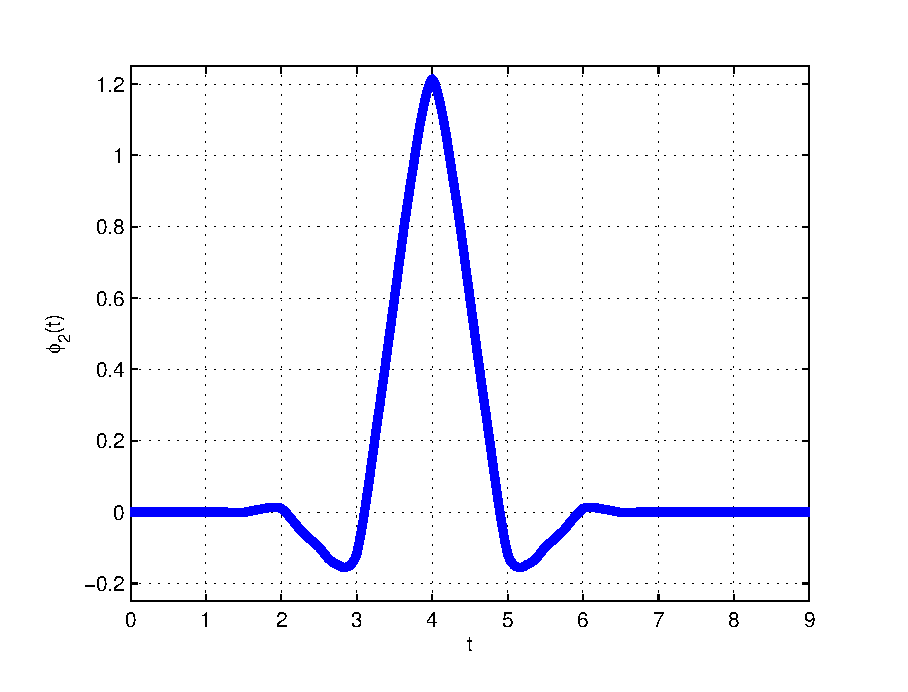
\includegraphics [width=0.45\textwidth]{./chap_3/bior_phi2}}} \hfill
		\subfloat[Synthesis wavelet function $ w_2(t) $]{\label{subfig3:bior_w2}{\includegraphics [width=0.45\textwidth]{./chap_3/bior_w2}}}\\
		\subfloat[Synthesis low-pass filter $ f_0 $]{\label{subfig3:bior_f0}{\includegraphics [width=0.45\textwidth]{./chap_3/bior_f0}}} \hfill
		\subfloat[Synthesis high-pass filter $ f_1 $]{\label{subfig3:bior_f1}{\includegraphics [width=0.45\textwidth]{./chap_3/bior_f1}}}\\
		\caption{Properties of `bior4.4' wavelet.}
		\label{fig3:bior_info}
		\end{figure}
